\subsection{Используем утилиту Synaptic}

\subparagraph{1) Что нужно было сделать?}

Проверьте, установлены ли у вас пакеты build-essential и manpages-dev при помощи утилиты Synaptic (Система > Администрирование > Менеджер пакетов Synaptic). Если не установлены - установите, они вам пригодятся.

\subparagraph{2) Как это сделали?}

\begin{MyVerbatimCode}[label=Debian terminal]
pavel-innokentevich-galanin@aspire-one-725:~$ sudo synaptic
\end{MyVerbatimCode}

Пакеты в Synaptic на~рисунках~\ref{fig:build-essential}~и~\ref{fig:manpages-dev}
(стр.~\pageref{fig:build-essential}~и~\pageref{fig:manpages-dev}).

\begin{figure}[!htp]
    \begin{minipage}{0.49\textwidth}
        \centering
        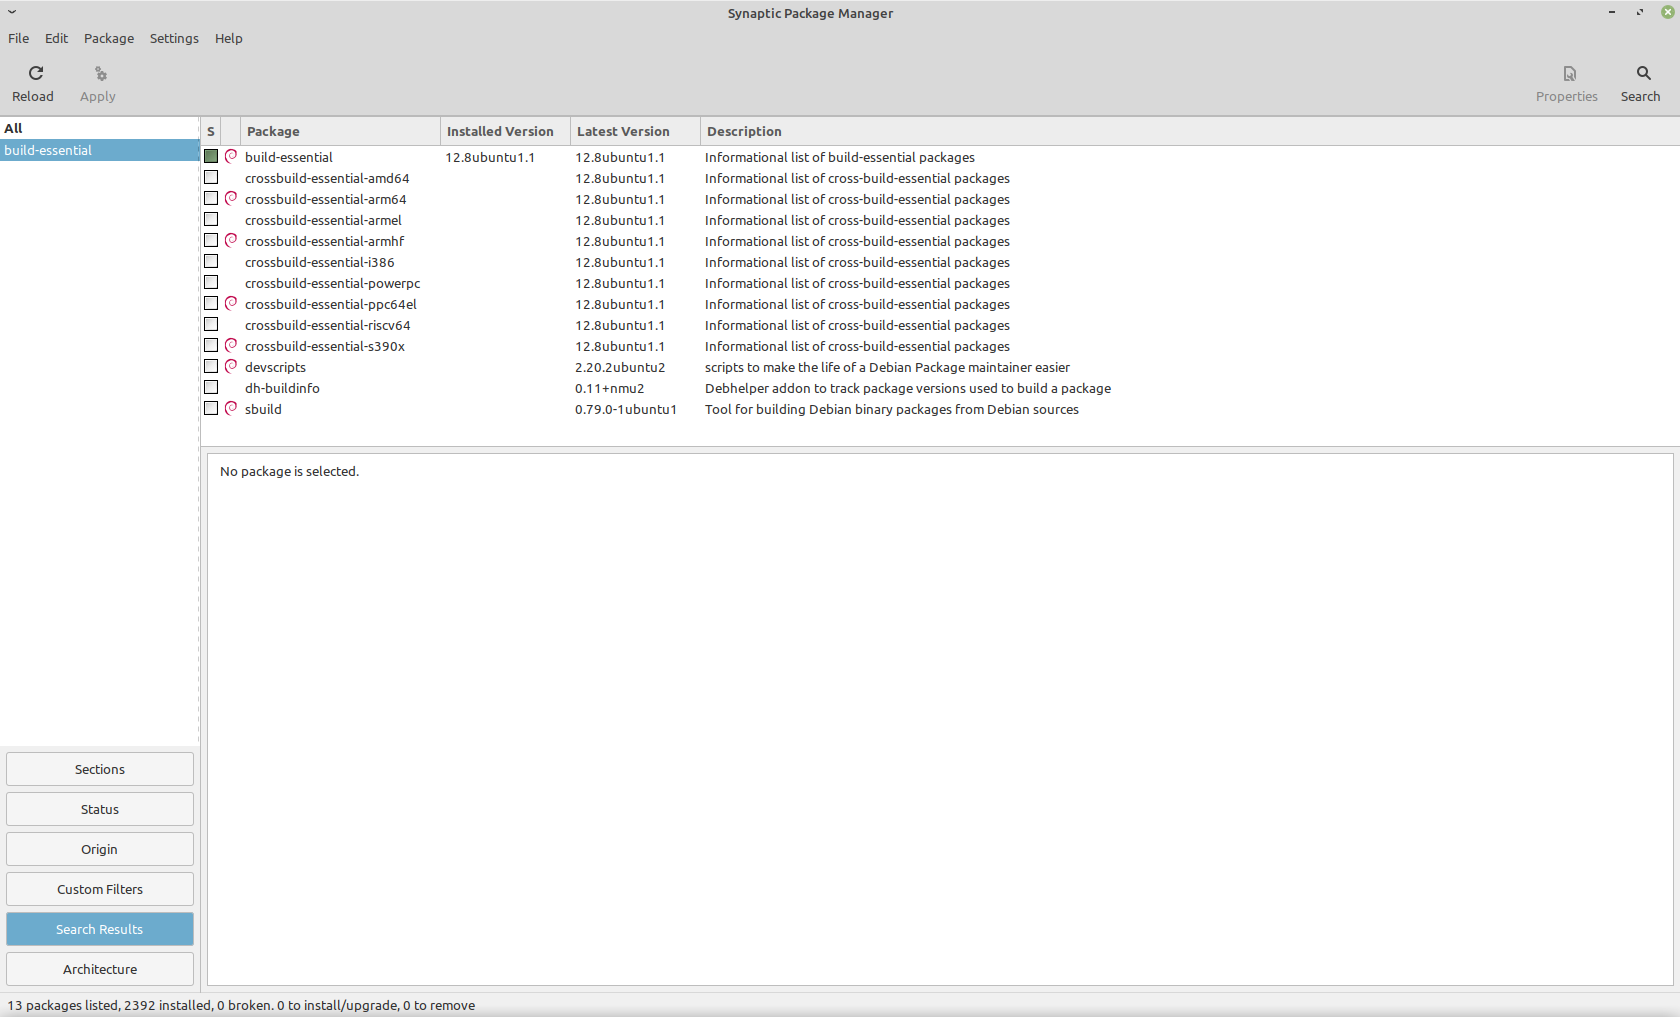
\includegraphics[width=\linewidth]
            {../input/task-2/2/build-essential.png}
        \caption{build-essential в Synaptic}
        \label{fig:build-essential}
    \end{minipage}
    \begin{minipage}{0.49\textwidth}
        \centering
        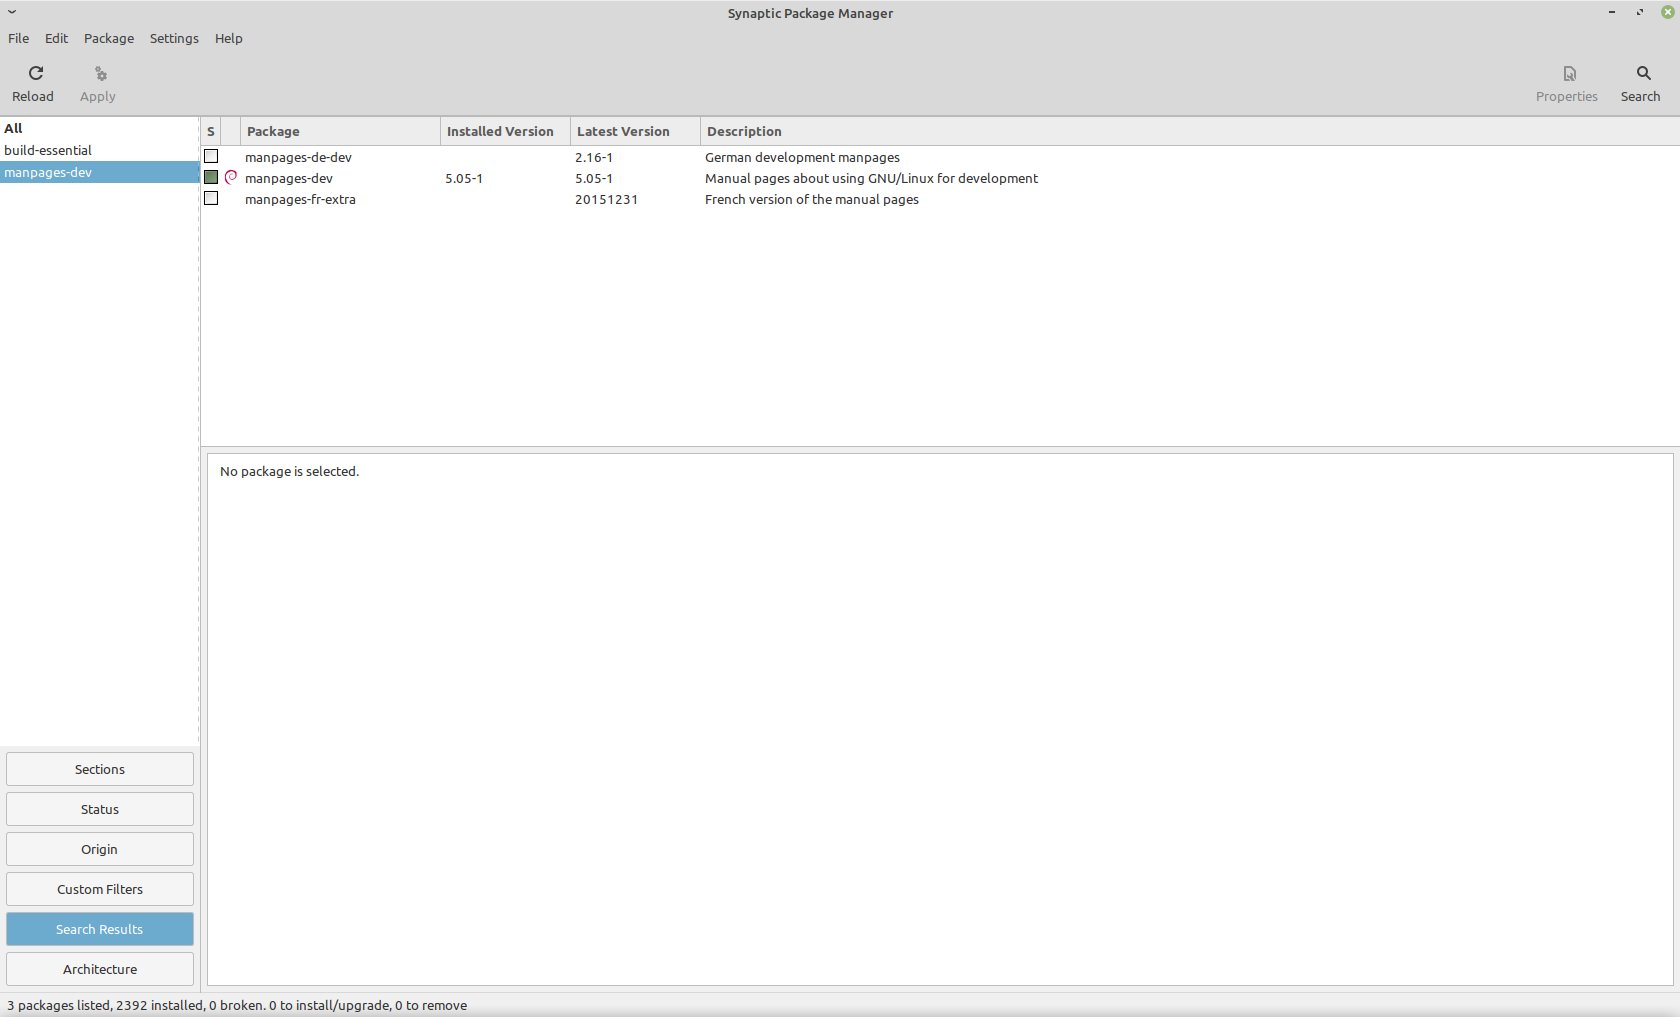
\includegraphics[width=\linewidth]
            {../input/task-2/2/manpages-dev.png}
        \caption{manpages-dev в Synaptic}
        \label{fig:manpages-dev}
    \end{minipage}
\end{figure}

\subparagraph{3) Что получилось?}

Открыли утилиту Synaptic. Через поиск проверили установленность пакетов.
